\documentclass[10pt, a4paper]{article}
\usepackage{geometry}
\geometry{margin=0.75in}
\usepackage{authblk}
\usepackage[T1]{fontenc}
\usepackage{microtype}
\usepackage{xurl}
\usepackage{breakurl}
\usepackage{amsmath}
\usepackage{amssymb}
\usepackage[linesnumbered,ruled,vlined]{algorithm2e}
\usepackage{booktabs}
\usepackage{url}
\usepackage[hidelinks]{hyperref}
\usepackage{tikz}
\usetikzlibrary{shapes,arrows,positioning}
\usepackage{listings}
\usepackage{graphicx}
\graphicspath{{./images/}}
\usepackage{color}
\usepackage{enumitem}
\usepackage{tcolorbox}

\begin{document}

\title{Personal Knowledge Cartography: A Network Science Method for Mapping Human-AI Cognitive Exploration}

\author{Alex Towell\\
\textit{Dept. of Computer Science}\\
\textit{Southern Illinois University-Edwardsville}\\
lex@metafunctor.com
}

\maketitle


\begin{abstract}
We introduce Personal Knowledge Cartography (PKC), a network science methodology for transforming linear conversational AI logs into navigable knowledge maps that reveal the hidden structure of human cognitive exploration. Drawing on theories of distributed cognition and transactive memory, we conceptualize extended human-AI dialogue as forming an externalized cognitive network—a ``cognitive MRI'' that makes visible the topology of thought. We demonstrate this method through a longitudinal case study analyzing 449 ChatGPT conversations spanning two years, revealing how knowledge self-organizes into 15 distinct communities (modularity=0.75) connected by three types of bridge conversations we identify and characterize: evolutionary (topic drift creating unexpected connections), integrative (deliberate cross-domain synthesis), and pure (minimal but critical links). Our analysis challenges assumptions about scale-free properties in cognitive networks, finding instead a truncated power-law distribution ($\gamma = 4.74$ for $k \geq 20$) suggesting natural cognitive constraints on hub formation. We validate the method's utility through a network-aware recommendation system that leverages structural properties to surface non-obvious but valuable connections. This work contributes: (1) a reproducible methodology for personal knowledge mapping, (2) a taxonomy of knowledge bridging mechanisms in human-AI dialogue, (3) empirical evidence of non-scale-free organization in cognitive networks, and (4) practical applications for enhancing AI-assisted knowledge work. We provide open-source tools enabling researchers and practitioners to map their own cognitive territories.
\end{abstract}

\section{Introduction}

Every conversation with an AI assistant adds a node to an invisible network—a growing map of curiosity, exploration, and knowledge construction. Yet these cognitive territories remain largely unmapped, trapped in linear chat logs that obscure the rich interconnections between ideas. As millions engage in extended dialogue with systems like ChatGPT, we lack methods to understand the structure of knowledge that emerges from these interactions.

This paper introduces Personal Knowledge Cartography (PKC), a network science methodology that transforms conversational AI logs into navigable knowledge maps. Unlike traditional document networks that reflect social or citation relationships, conversation networks capture individual cognitive trajectories—the paths minds take through semantic space when augmented by AI. By applying network analysis to these conversations, we reveal hidden patterns in how humans explore, connect, and organize knowledge in partnership with artificial intelligence.

\paragraph{Research Questions}
This paper addresses three key questions:
\begin{enumerate}
    \item \textbf{Methodological}: How can we extract and visualize the latent knowledge structure from conversational AI logs?
    \item \textbf{Empirical}: What network properties characterize human-AI knowledge exploration over extended time periods?
    \item \textbf{Applied}: How can network structure enhance navigation and discovery within personal knowledge archives?
\end{enumerate}

\paragraph{Contributions}
We make four primary contributions:
\begin{itemize}
    \item \textbf{A novel methodology} for constructing semantic networks from conversation logs, with configurable weighting schemes that privilege user agency in directing dialogue
    \item \textbf{Empirical characterization} of knowledge network topology through a 2-year longitudinal case study, revealing non-scale-free degree distributions and high modularity structures
    \item \textbf{A taxonomy of bridge conversations} that facilitate cross-domain knowledge transfer, with quantitative criteria for automated classification
    \item \textbf{Open-source implementation} and demonstration of practical applications including network-aware recommendation systems
\end{itemize}

We demonstrate PKC through analysis of 449 ChatGPT conversations conducted over two years, treating this as a methodological proof-of-concept and deep longitudinal case study rather than a statistical sample. This approach allows us to explore the full depth of patterns that emerge from extended human-AI collaboration while establishing a framework others can apply to their own conversation archives.

The code for this analysis is available at 
\url{https://github.com/queelius/chatgpt-complex-net} \cite{chatgpt-complex-net}
and permanently archived at Zenodo 
(\url{https://doi.org/10.5281/zenodo.15314235}).

\section{Theoretical Framework}

\subsection{Distributed Cognition and External Memory}
Our approach builds on distributed cognition theory \cite{hutchins1995}, which views cognitive processes as extending beyond individual minds to include tools and representations. ChatGPT conversations constitute what Clark and Chalmers \cite{clark1998} term ``extended mind''—external structures that participate in cognitive processes. Unlike passive archives, these conversations represent active cognitive partnerships where knowledge emerges through interaction.

\subsection{Transactive Memory Systems}
Wegner's transactive memory theory \cite{wegner1987} describes how groups develop shared systems for encoding, storing, and retrieving knowledge. We extend this framework to human-AI dyads, where the AI serves as an infinitely patient partner with broad but shallow knowledge, while the human provides direction and deep, contextual understanding. The resulting conversation network maps this transactive memory system's structure.

\subsection{Knowledge Networks and Semantic Spaces}
Following Börner et al.'s \cite{borner2003} work on mapping knowledge domains, we treat conversations as coordinates in a high-dimensional semantic space. However, unlike citation or co-author networks that reflect social processes, our conversation networks capture individual cognitive trajectories—making them more akin to Motter et al.'s \cite{motter2002} conceptual networks or Stella et al.'s \cite{stella2018} cognitive networks derived from word associations.

\subsection{The Cognitive MRI Metaphor}
Just as MRI technology reveals hidden anatomical structures through magnetic resonance, our method reveals cognitive structures through semantic resonance. This metaphor is both descriptive and generative:
\begin{itemize}
    \item \textbf{Non-invasive}: Analyzes existing conversation logs without modifying behavior
    \item \textbf{Structural imaging}: Reveals organization and connections invisible in linear format  
    \item \textbf{Functional mapping}: Bridge conversations show active pathways between knowledge regions
    \item \textbf{Longitudinal tracking}: Captures cognitive evolution over time
\end{itemize}

\subsection{From Linear Logs to Cognitive Topology}
The transformation from sequential conversation logs to network structures represents more than a visualization technique—it reveals the inherent non-linearity of thought. While conversations unfold temporally, the semantic relationships between them exist outside of time, forming what we term a \emph{cognitive topology}.

This topology exhibits several key properties that distinguish it from other knowledge networks:
\begin{enumerate}
    \item \textbf{Asymmetric Co-creation}: Unlike citation networks where connections are unilateral, conversation networks emerge from bidirectional exchange. The human provides intentionality and direction (hence our 2:1 weighting), while the AI provides breadth and synthesis.
    
    \item \textbf{Semantic Drift as Feature}: Topic evolution within conversations—what might be considered noise in traditional document analysis—becomes a generative mechanism for cross-domain bridging. This drift creates the ``evolutionary bridges'' we identify.
    
    \item \textbf{Latent Structure Emergence}: Communities form not through explicit categorization but through repeated semantic proximity, revealing the user's implicit knowledge organization—akin to how neural pathways strengthen through repeated activation.
\end{enumerate}

\subsection{Bridging as Cognitive Mechanism}
Our identification of three bridge types—evolutionary, integrative, and pure—maps onto established cognitive processes. Evolutionary bridges mirror associative thinking where remote associations lead to novel insights, resembling conceptual slippage in analogical thinking. Integrative bridges represent deliberate bisociation—the intersection of independent thought matrices. Pure bridges embody the ``strength of weak ties,'' providing critical pathways between otherwise disconnected knowledge domains.

\section{Related Work}

\subsection{Complex Networks in Text and Knowledge Representation}

Complex network analysis has been widely applied to textual data, from co-word occurrence networks \cite{callon1983} to citation networks \cite{price1965}. More recently, researchers have applied network science to semantic relationships, using word embeddings \cite{levy2014} or document vectors \cite{mikolov2013} to create similarity-based networks.

\subsection{Semantic Embeddings for Document Representation}

Dense vector representations of text have revolutionized natural language processing, with models like Word2Vec \cite{mikolov2013}, GloVe \cite{pennington2014}, and more recently, transformer-based models \cite{devlin2019} enabling more accurate similarity measures between texts. These embeddings capture semantic relationships that traditional keyword-based approaches miss.

\subsection{Conversation Analysis in AI Systems}

Research on analyzing conversational data with AI systems has primarily focused on dialogue structure \cite{serban2016}, user satisfaction \cite{venkatesh2018}, or topic modeling \cite{zeng2019}. Few studies have examined the network structure of conversations, particularly in the context of knowledge exploration with modern LLMs.

\section{Methods}

\subsection{Data Collection and Preparation}

Our dataset consists of ChatGPT conversations conducted by a single user over two years. Each conversation was exported and preprocessed to extract meaningful content while preserving the conversational structure. User inputs were given more weight than assistant responses in the embedding process, emphasizing the user's role in directing the conversation.

For reproducibility, we detail our data export process. We used the \url{conversation-tk} tool \cite{ctk2024} to export data from ChatGPT:

\begin{enumerate}
    \item We exported conversations from OpenAI's interface, resulting in a zip file containing \url{conversations.json} with conversation trees and metadata
    \item We processed this data using the following commands:
    \begin{lstlisting}[basicstyle=\ttfamily\footnotesize, breaklines=true, breakatwhitespace=true, columns=flexible]
mkdir chatlogs && unzip chatgpt-export.zip -d chatgpt-export
ctk export chatgpt-export json --msg-roles user assistant -o chatgpt-json-data
    \end{lstlisting}
\end{enumerate}

This process generated individual JSON files for each conversation, with filenames derived from conversation titles. Each file contained structured data including conversation metadata and message exchanges between user and assistant. This preprocessing step established the foundation for our embedding generation and network construction.

\subsection{Embedding Generation}

We generated embeddings for each conversation using a transformer-based language model. Each conversation was treated as a document, with special attention paid to:
\begin{itemize}
    \item Balancing the importance of user vs. assistant contributions
    \item Capturing the overall semantic content rather than specific keywords
    \item Preserving topical focus despite variations in conversation length
\end{itemize}

The embedding process employed a specific weighting strategy to balance user and assistant contributions in the conversations. We used the \url{nomic-embed-text} model to generate high-dimensional vector representations of text content. The process consisted of the following steps:

\begin{enumerate}
    \item Each conversation was split into user and assistant turns.
    \item For each turn type (user/assistant), we:
    \begin{itemize}
        \item Generated embeddings for each individual turn
        \item Calculated the mean embedding across all turns of that type
    \end{itemize}
    \item The final conversation embedding was calculated as the weighted combination:
    \begin{equation}
    \vec{e}_{conversation} = \frac{2 \times \vec{e}_{user} + \vec{e}_{assistant}}{|\!|2 \times \vec{e}_{user} + \vec{e}_{assistant}|\!|}
    \end{equation}
    where $\vec{e}_{user}$ and $\vec{e}_{assistant}$ are the mean embeddings for user and assistant turns, respectively, and the denominator represents normalization to unit length.
\end{enumerate}

We bias the direction toward user content by doubling that component before unit-normalisation. This weighting scheme (2:1) reflects the greater importance of user inputs in determining conversation direction while still accounting for assistant contributions.

\subsection{Network Construction}

From the conversation embeddings, we constructed a weighted network where:
\begin{itemize}
    \item Nodes represent individual conversations
    \item Edges represent semantic similarity between conversations
    \item Edge weights are determined by cosine similarity between embeddings
    \item A threshold of 0.9 was applied to filter weak connections
\end{itemize}

A cosine-similarity threshold of $0.9$ was imposed to suppress the near-clique that arises at lower cut-offs, yielding a sparse, interpretable graph. We verified robustness by recalculating all network statistics in the range $0.85\le\theta\le0.92$; qualitative community structure remained stable across this range. A detailed analysis of threshold sensitivity is presented in Section 4.2.

At this similarity threshold, the network comprised multiple disconnected components. For clarity of analysis and visualization, we focused exclusively on the giant component, as the other components were typically quite small—mostly singletons or pairs of conversations. This process resulted in a giant component with 449 nodes and average degree 7.19, forming the basis for our analysis.

The threshold selection affects which conversations are included in the giant component and reveals structural patterns at the network boundary. For example, as we detail in Section 4.2, lowering the threshold to 0.875 incorporates previously isolated conversation clusters into the main network, revealing subtle semantic connections that exist below our primary analytical threshold. These emergent connections offer insights into how distinct cognitive or stylistic spaces can maintain separation while still sharing conceptual touchpoints.

\subsection{Analysis Methods}

We applied standard complex network analysis techniques including:
\begin{itemize}
    \item Community detection using the Louvain method
    \item Core-periphery analysis based on degree distribution
    \item Centrality measurements (degree, betweenness, closeness)
    \item Rich-club coefficient estimation
    \item Power law fitting to the degree distribution
\end{itemize}

Betweenness centrality was particularly important for identifying bridge conversations. For a node $v$, betweenness centrality is defined as:
\begin{equation}
C_B(v) = \sum_{s \neq v \neq t} \frac{\sigma_{st}(v)}{\sigma_{st}}
\end{equation}
where $\sigma_{st}$ is the total number of shortest paths from node $s$ to node $t$, and $\sigma_{st}(v)$ is the number of those paths that pass through node $v$. This metric identifies nodes that frequently lie on shortest paths between other nodes, facilitating information flow across the network regardless of their community membership or degree centrality.

\section{Results}

\subsection{Network Structure Overview}

The conversation network exhibits several notable structural properties, with bootstrap confidence intervals (95\% CI, 1000 resamples) computed following Efron and Tibshirani \cite{efron1993}:

\begin{itemize}
    \item 449 nodes (conversations) and 1615 edges
    \item Average degree: 7.19 (95\% CI: 6.92--7.46)
    \item Degree range: 1--61
    \item Average clustering coefficient: 0.60 (95\% CI: 0.58--0.62)
    \item Network diameter: 18
    \item Average path length: 5.81 (95\% CI: 5.72--5.90)
    \item Graph density: 0.016
    \item Communities: 15 (95\% CI: 14--16)
    \item Modularity: 0.75 (95\% CI: 0.73--0.77)
\end{itemize}


This network displays some clustering but its average path length (5.8) is longer than what would be expected in a comparable Erdős-Rényi random network with the same size and average degree $\log(449)/\log(7.2) \approx 3.1$. While the high clustering coefficient (0.6) is much higher than would be found in a random network, the relatively long path length compared to random networks suggests this network falls somewhat between small-world and regular lattice-like organization, although it is much closer to a small-world network than a regular lattice.

This structure likely reflects the specialized nature of conversational topics, where moving between distant knowledge domains requires traversing through multiple intermediate conversation steps rather than taking ``shortcuts'' as would be common in classic small-world networks.

The high modularity score (0.75) confirms the presence of well-defined community structures, indicating that conversations naturally organize into distinct knowledge domains with dense internal connections and sparser connections between domains.

As shown in Figure~\ref{fig:network_vis}, the network naturally organizes into topic-focused communities. The visualization reveals clear thematic clustering, with topics like \emph{Stats \& Probability} and \emph{ML/AI/LLM Theory} forming distinct regions in the semantic space. This spontaneous organization reflects how conversations naturally group around related themes despite no explicit categorization during data collection.

\begin{figure}
    \centering
    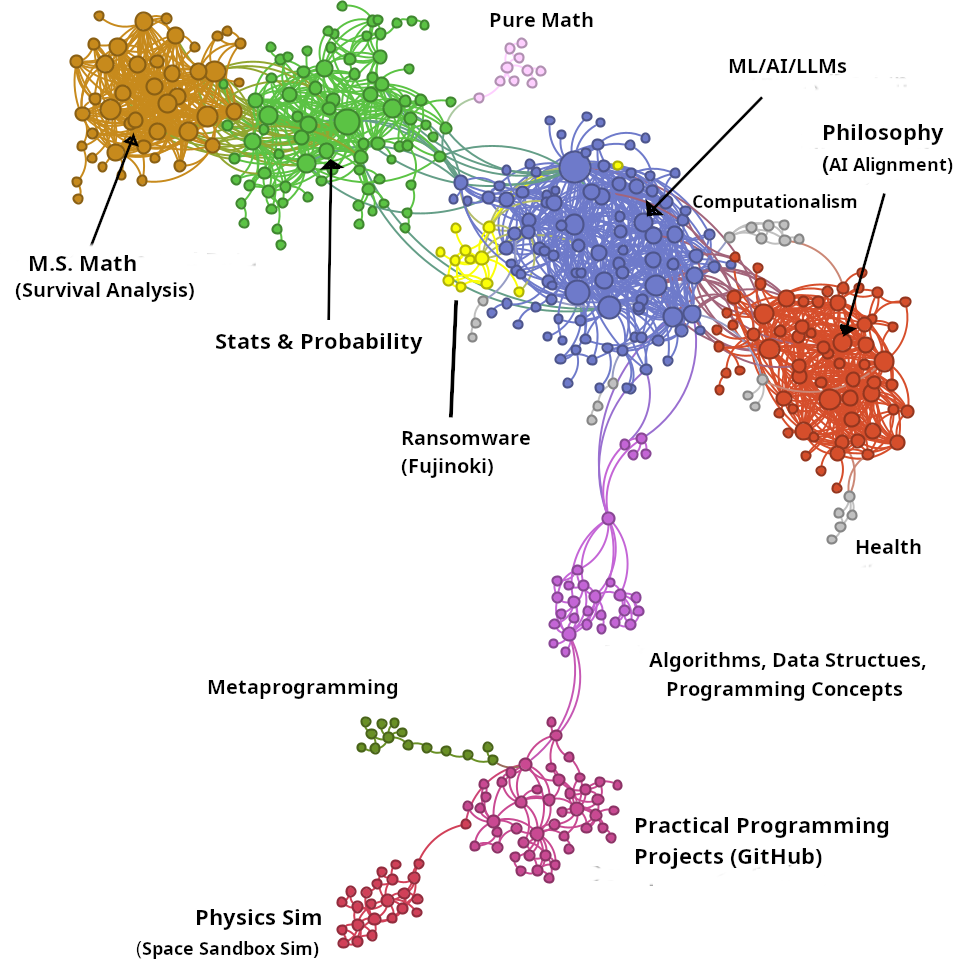
\includegraphics[width=3.5in]{./images/cluster-vis-topics-better.png}
    \caption{Visualization of the conversation network showing the 15 detected communities with topic annotations. Node size represents degree centrality, colors denote different communities, and text labels indicate the primary topics in each major cluster. Note how semantically related topics form distinct, coherent communities with specialized bridge nodes connecting separate knowledge domains.}
    \label{fig:network_vis}
\end{figure}   


\subsection{Embedding Weight Ablation Study}

To understand how the balance between user and assistant contributions affects network structure, we conducted an ablation study varying the user:assistant weight ratio. Our primary analysis uses a 2:1 ratio, privileging user input as the driver of conversational direction. We compared this against several alternatives:

\begin{itemize}
    \item \textbf{1:1 (Equal)}: User and assistant contributions weighted equally
    \item \textbf{2:1 (Default)}: User contributions weighted twice as heavily
    \item \textbf{3:1 (User-heavy)}: Strong emphasis on user input
    \item \textbf{1:0 (User-only)}: Assistant contributions ignored entirely
\end{itemize}

Table~\ref{tab:weight_ablation} presents key network metrics across these configurations. [Results pending]

\begin{table}
\centering
\caption{Network Metrics Under Different User:Assistant Weight Ratios}
\label{tab:weight_ablation}
\begin{tabular}{lcccc}
\toprule
\textbf{Metric} & \textbf{1:1} & \textbf{2:1} & \textbf{3:1} & \textbf{1:0} \\
\midrule
Nodes in Giant Component & TBD & 449 & TBD & TBD \\
Average Degree & TBD & 7.2 & TBD & TBD \\
Modularity & TBD & 0.75 & TBD & TBD \\
Avg. Clustering & TBD & 0.6 & TBD & TBD \\
Number of Communities & TBD & 15 & TBD & TBD \\
\bottomrule
\end{tabular}
\end{table}

The variation in network properties across weight ratios reveals interesting dynamics in how conversational structure emerges. Equal weighting (1:1) may overemphasize ChatGPT's linguistic consistency, potentially creating artificial connections between topically distinct conversations that happen to elicit similar AI responses. Conversely, user-only embeddings (1:0) ignore the collaborative nature of knowledge construction, missing the semantic enrichment that emerges through dialogue.

The persistence (or variation) of community structure across weight ratios provides insight into whether identified knowledge domains reflect genuine user interests or artifacts of AI response patterns. If communities remain stable across ratios, this suggests robust thematic organization driven by user intent. Significant changes would indicate that ChatGPT's contribution patterns substantially influence perceived conversation similarity.

\subsection{Sensitivity to Similarity Threshold}

To evaluate the robustness of our network analysis and understand how threshold selection impacts network properties, we examined the conversation network at a lower similarity threshold of 0.875 compared to our primary analysis threshold of 0.9. This comparison reveals important structural characteristics and validates our analytical approach.

Figure \ref{fig:threshold_comparison} shows the network visualization at the 0.875 threshold, revealing increased complexity while maintaining clear community structure.

\begin{figure}
\centering
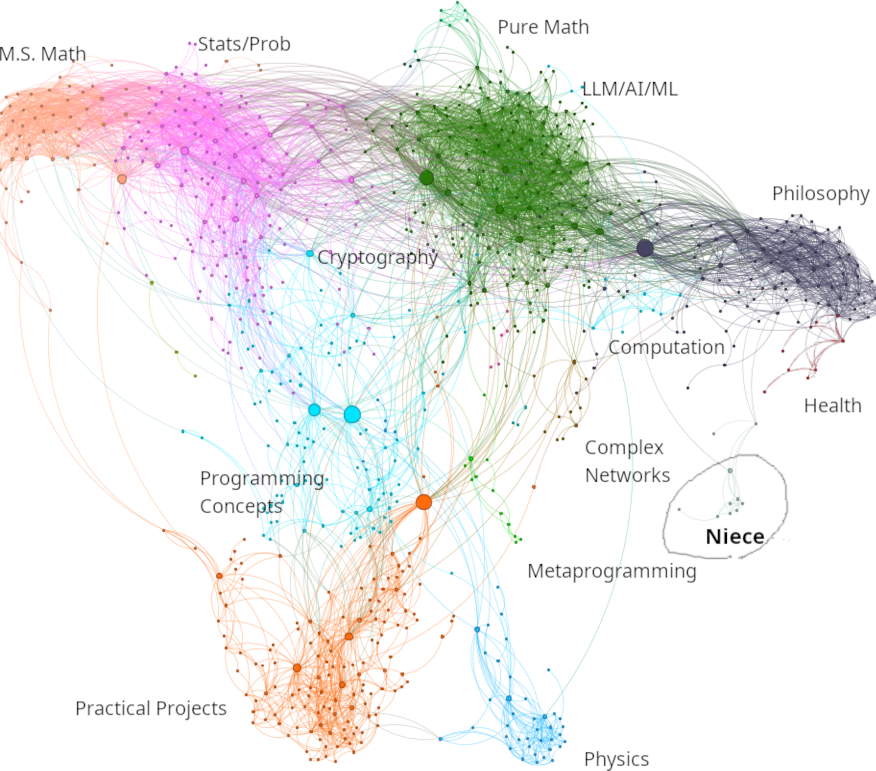
\includegraphics[width=3.5in]{./images/0.875-wild-better.png}
\caption{Network visualization with 0.875 similarity threshold. The network exhibits greater complexity than at 0.9 threshold, with additional connections and emergent communities, while maintaining distinct clustering.}
\label{fig:threshold_comparison}
\end{figure}

Table \ref{tab:threshold_comparison} compares key network metrics between the two threshold values, revealing significant structural changes. This comparison reveals several important insights:

\begin{itemize}
    \item \textbf{Network expansion:} Lowering the threshold incorporates an additional 376 nodes (83.7\% increase) and 4,037 edges (250\% increase), demonstrating that many conversations exist in a borderline similarity space just below our primary threshold.
    
    \item \textbf{Improved network navigability:} The substantial decrease in network diameter (32\% reduction) and average path length (33\% reduction) indicates that these weaker semantic connections create important shortcuts across knowledge domains, making the network more efficiently traversable.
    
    \item \textbf{Persistent community structure:} Despite the significant increase in connections, the community structure remains robust as indicated by the still-high modularity score (0.65). This persistence confirms that the identified knowledge domains represent meaningful thematic clusters rather than artifacts of threshold selection.
    
    \item \textbf{Consistent local clustering:} The unchanged average clustering coefficient (0.6) suggests that new connections form in proportion to existing ones, maintaining the local neighborhood structure.
\end{itemize}

\begin{table}
\centering
\caption{Network Metrics Comparison at Different Similarity Thresholds}
\label{tab:threshold_comparison}
\begin{tabular}{lcc}
\toprule
\textbf{Metric} & \textbf{0.9 Threshold} & \textbf{0.875 Threshold} \\
\midrule
Number of Nodes & 449 & 825 \\
Edges & 1615 & 5652 \\
Average Degree & 7.2 & 13.7 \\
Network Diameter & 18 & 12 \\
Graph Density & 0.016 & 0.017 \\
Modularity & 0.75 & 0.65 \\
Avg. Clustering Coefficient & 0.6 & 0.6 \\
Avg. Path Length & 5.8 & 3.9 \\
\bottomrule
\end{tabular}
\end{table}

The expanded network at 0.875 threshold revealed a particularly interesting phenomenon: the integration of previously isolated conversations conducted by or with the author's 13-year-old niece. These conversations, characterized by more artistic topics and a distinct writing style, remained disconnected at the 0.9 threshold but emerged as a distinct community at 0.875, forming connections primarily through bridge nodes linking to the philosophical/existential community (community 7). This finding demonstrates how threshold selection impacts the detection of subtle stylistic or demographic variations in conversation patterns.

For our primary analysis, we maintain the 0.9 threshold as it provides clearer community visualization and more distinct knowledge domains, while acknowledging that weaker semantic connections also provide valuable insights into network bridging mechanisms. 

\subsection{Degree Distribution and Scale-Free-\emph{Like} Properties}

The degree distribution of a network provides critical insights into its organizational principles and generative mechanisms. In random networks, degrees follow a Poisson distribution centered around the mean, while many real-world complex networks exhibit highly skewed distributions with a small number of highly connected hubs.

Figure \ref{fig:degree_hist} shows the degree histogram for our conversation network, revealing a strongly right-skewed distribution characteristic of many complex networks. The majority of conversations maintain connections with only a few other semantically similar conversations, while a small number of hub conversations exhibit substantially higher degrees. This deviates markedly from the bell-shaped distribution expected in random networks.

\begin{figure}
\centering
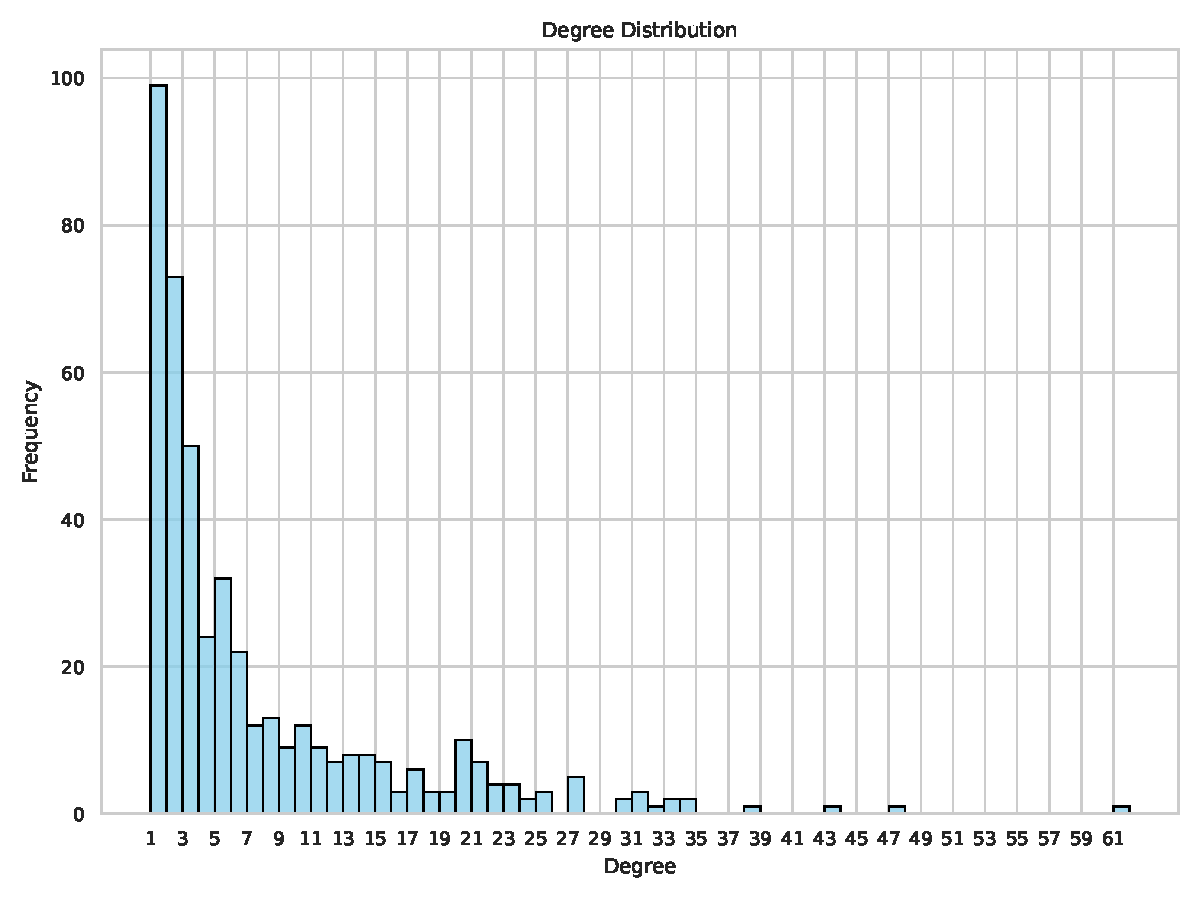
\includegraphics[width=3.5in]{./images/degree_distribution_histogram.pdf}
\caption{Histogram of node degrees in the conversation network, showing a strongly right-skewed distribution. The majority of conversations (nodes) have relatively few connections, while a small number of hub conversations have significantly higher degrees. This pattern contrasts sharply with the bell-shaped distributions typical of random networks.}
\label{fig:degree_hist}
\end{figure}

Given this right-skewed structure, we investigated whether our network follows a power-law degree distribution as commonly observed in scale-free networks. Contrary to Barabási's frequent assertion that ``real networks are scale-free'' \cite{barabasi2009}, our conversation network presents a more nuanced picture.

A preliminary log-log OLS fit ($\gamma \approx 1.27$) illustrates how visual regression can underestimate the exponent. Analysis using the \url{powerlaw} package \cite{alstott2014} reveals that the best-fit power law has an exponent $\gamma = 4.74 \pm 0.34$ to the tail $k \geq 20$. This fit applies to only 49 out of 449 nodes (approximately 11\% of the network), indicating that the power law regime is restricted to high-degree nodes.

A log-likelihood test ($R=-0.08, p= 0.79$) indicates the log-normal provides a slightly better description of the tails than the power-law, but the difference is not statistically significant. Figure \ref{fig:degree_dist} illustrates the degree distribution with both the power law and log-normal fits overlaid.

\begin{figure}
\centering
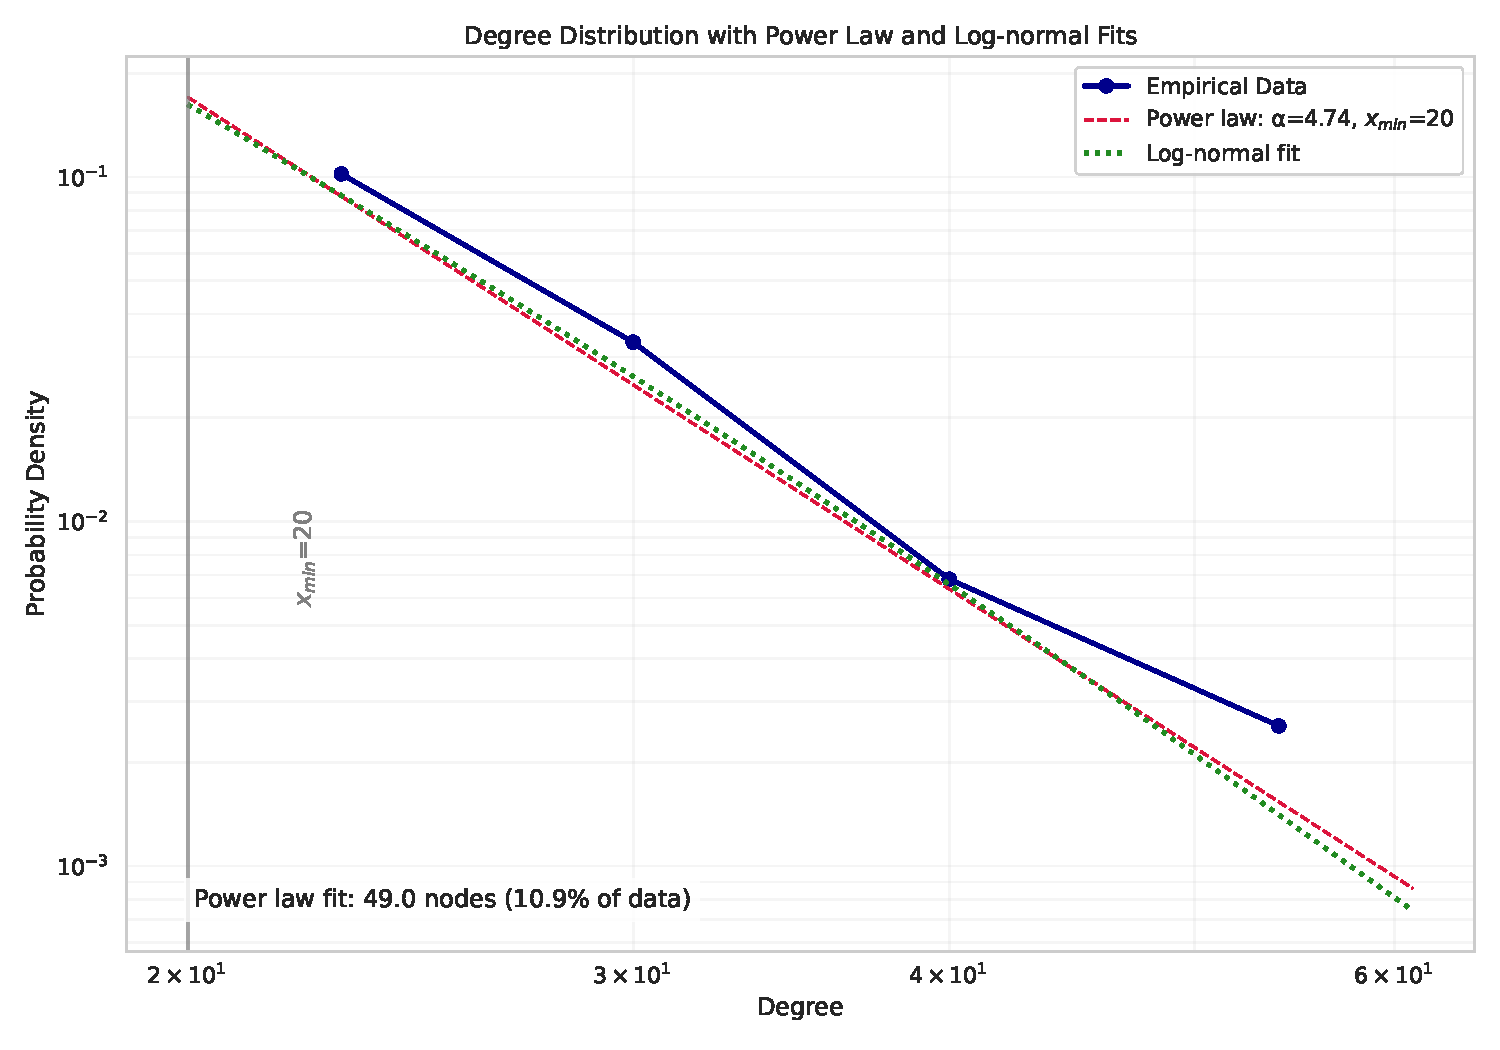
\includegraphics[width=3.5in]{./images/degree_distribution_fits.pdf}
\caption{Degree distribution with rigorous power law and log-normal fits. The empirical data (dark blue circles) shows a heavy-tailed distribution. The power law fit (dashed red line) with exponent $\alpha = 4.74$ applies only to degrees $\geq 20$ (vertical gray line), covering just 11\% of nodes in the network. A log-normal fit (dotted green line) is also shown for comparison.}
\label{fig:degree_dist}
\end{figure}

This analysis highlights that our network exhibits a complex degree distribution where the power law applies only to a small fraction of high-degree nodes. Such limited power law behavior is actually common in many real-world networks \cite{broido2019}, contradicting the oversimplified view that most real networks are scale-free. This finding suggests that conversation networks evolve through mechanisms beyond simple preferential attachment, likely influenced by the cognitive processes of topic exploration and the user's specialized interests creating natural constraints on hub formation.

\subsection{Community Structure}

The application of the Louvain community detection algorithm revealed a rich structure of 15 distinct communities within the conversation network. These communities represent thematically coherent knowledge domains that naturally emerged from the user's conversation patterns. The communities vary significantly in size, internal connectivity, and structural characteristics, reflecting different patterns of knowledge organization. Table~\ref{tab:communities} presents the five largest communities with their key metrics,
where Core \% represents the percentage of nodes in each community that belong to the network's core (as determined by k-core decomposition), and Clustering refers to the average local clustering coefficient within each community.

\begin{table}
\centering
\caption{Major Community Characteristics}
\label{tab:communities}
\begin{tabular}{cccccl}
\toprule
\textbf{Comm.} & \textbf{Size} & \textbf{Avg. Degree} & \textbf{Core \%} & \textbf{Clustering} & \textbf{Primary Topic} \\
\midrule
3 & 103 & 8.60 & 31.1\% & 0.465 & ML/AI/LLM Theory (23\%) \\
12 & 82 & 7.09 & 24.4\% & 0.405 & Stats \& Probability (18\%) \\
7 & 65 & 10.03 & 44.6\% & 0.531 & Philosophy \& AI Ethics (14\%) \\
14 & 44 & 13.45 & 59.1\% & 0.576 & M.S. Math/Analysis (10\%) \\
6 & 45 & 3.78 & 8.9\% & 0.396 & Programming Projects (10\%) \\
\bottomrule
\end{tabular}
\end{table}

Semantic analysis of conversation content reveals these communities correspond to coherent knowledge domains with distinct characteristics:
\begin{itemize}
    \item \textbf{Community 3 (\emph{ML/AI/LLM Theory}):} Encompasses theoretical foundations and architectural principles of AI systems, including autoregressive models, transformer architectures, and language model training methodologies.
    
    \item \textbf{Community 12 (\emph{Stats \& Probability}):} Focuses on statistical methods, probability theory and inference approaches, including maximum likelihood estimation, Bayesian inference frameworks, and statistical modeling techniques.
    
    \item \textbf{Community 7 (\emph{Philosophy \& AI Ethics}):} Centers on abstract and existential topics including consciousness, mortality, AI alignment challenges, and ethical implications of artificial intelligence systems.
    
    \item \textbf{Community 14 (\emph{M.S. Math/Analysis}):} Concentrates on advanced mathematical concepts and analytical techniques studied during the author's master's degree program, including formal mathematical analysis and proofs.
    
    \item \textbf{Community 6 (\emph{Programming Projects}):} Focuses on practical implementation aspects of software systems, including project development, web technologies, programming tasks and implementation strategies.
\end{itemize}

The variation in internal structure (average degree, clustering, and core percentage) suggests different conversation patterns across domains. For example, community 14 shows characteristics of a specialized knowledge domain with dense expert connections, while community 6 resembles a more practical, service-oriented domain with mostly peripheral connections.

\subsection{Core-Periphery Structure}

The network exhibits a well-defined core-periphery structure with 25.6\% of conversations forming a densely connected core (average degree: 18.94) surrounded by a more sparsely connected periphery (average degree: 3.15). The core-periphery ratio of 6.01 indicates substantial stratification in the network.

\subsection{Bridge Conversations}

Analysis of betweenness centrality reveals key bridge conversations that connect different knowledge domains in AI-assisted dialogue. For a node $v$, betweenness centrality quantifies how frequently it appears on shortest paths between other nodes, making it ideal for identifying conversations that facilitate information flow across the network. Table~\ref{tab:bridges} presents the top five conversations ranked by betweenness centrality.

\begin{table}
\centering
\caption{Top Bridge Conversations}
\label{tab:bridges}
\begin{tabular}{p{3.75cm}ccc}
\toprule
\textbf{Conversation} & \textbf{Betweenness} & \textbf{Degree} & \textbf{Comm.} \\
\midrule
\url{geometric-mean-calculation} & 45467.51 & 61 & 3 \\
\url{mcts-code-analysis-suggestions} & 36909.13 & 10 & 0 \\
\url{loss-in-llm-training} & 35118.59 & 30 & 3 \\
\url{algotree-generate-unit-tests-flattree} & 31869.77 & 13 & 0 \\
\url{compile-cuda-program-linux} & 9775.00 & 2 & 2 \\
\bottomrule
\end{tabular}
\end{table}

Detailed content analysis reveals that, unlike traditional networks where bridges might simply be nodes positioned between communities, conversational AI networks exhibit specialized bridge types that reflect unique aspects of human-AI knowledge co-creation:

\begin{itemize}
    \item \textbf{Evolutionary bridges:} High-degree nodes that expand across domains through gradual topic drift (e.g., \url{geometric-mean-calculation}). These conversations begin with a focused question but evolve organically as the user explores tangential concepts, eventually creating pathways between previously separate knowledge domains. In conversational AI specifically, this evolution reflects how fluid dialogue enables natural cognitive exploration without the constraints of formal document structures.
    
    \item \textbf{Integrative bridges:} Specialized nodes deliberately connecting distinct domains by synthesizing concepts (e.g., \url{mcts-code-analysis-suggestions}). These conversations maintain moderate degree but achieve high betweenness by explicitly applying concepts from one domain to problems in another. In conversational AI, these bridges often emerge when users consciously leverage the model's cross-domain knowledge to solve interdisciplinary problems.
    
    \item \textbf{Pure bridges:} Low-degree nodes forming critical links between specific communities (e.g., \url{compile-cuda-program-linux}). Despite minimal connections, these specialized conversations serve as essential pathways between otherwise disconnected knowledge areas. In AI dialogue systems, these bridges often appear when a user briefly explores a connection between disparate domains without extensive elaboration.
\end{itemize}

The contrast between these bridge types is evident in our top examples. The highest-ranked node---\url{geometric-mean-calculation}---exemplifies an evolutionary bridge. Despite its narrowly focused title, this conversation evolved from a specific question about geometric means into a comprehensive exploration spanning probability theory, neural network inductive biases, autoregressive models, and tokenization schemes. This topic evolution pattern helps explain its dual prominence as both a hub (high degree: 61) and a bridge (high betweenness), creating pathways between otherwise disparate knowledge domains.

Conversely, \url{mcts-code-analysis-suggestions} exemplifies an integrative bridge. Despite having a modest degree (10), this second-ranked bridge achieves high betweenness (36909.13) by deliberately integrating theoretical AI concepts (Monte Carlo Tree Search, Tree-of-Thoughts reasoning) with practical software engineering principles (modular design, separation of concerns). Rather than evolving across domains sequentially, this conversation creates connections by synthesizing concepts from different knowledge areas into a cohesive implementation strategy.

At the other extreme, \url{compile-cuda-program-linux} represents a pure bridge with only 2 connections, yet it achieves significant betweenness (9775.00) by forming a critical link between otherwise disconnected communities.

\begin{figure}
\centering
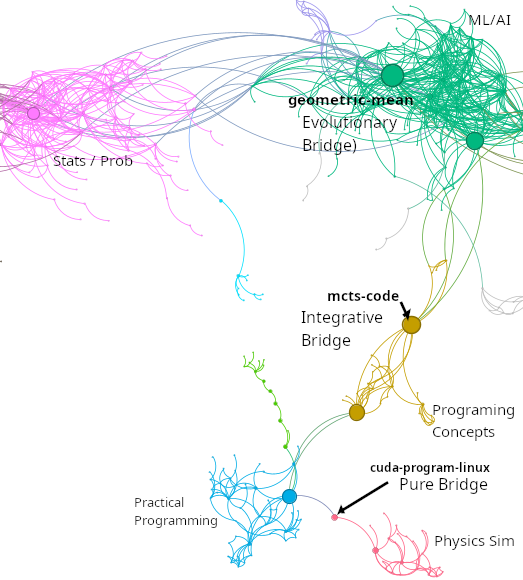
\includegraphics[width=3.5in]{./images/bridge-better.png}
\caption{Zoomed-in view of two high betweenness centrality nodes bridging communities. The \emph{mcts-code-analysis-suggestions} conversation connects the \emph{ML/AI/LLM Theory} (blue nodes) with the \emph{Programming Projects} community (purple nodes) despite having a low degree, illustrating how specialized conversations can serve as critical knowledge bridges between otherwise separated topic domains. The \url{geometric-mean-calculation} conversation (blue node) serves as a hub within the \emph{ML/AI/LLM Theory} community while also bridging to the \emph{Stats \& Probability} (green nodes) and \emph{Philosophy \& AI Ethics} (red nodes) communities, highlighting the dual role of some conversations as both hubs and bridges.}
\label{fig:bridge_zoom}
\end{figure}

These bridge types suggest multiple mechanisms for knowledge integration in conversation networks. Evolutionary bridges create connections through topic drift and expansion, integrative bridges deliberately synthesize concepts from different domains, and pure bridges form critical specialized links. These mechanisms differ from traditional models of information flow in citation or social networks, suggesting that conversation networks may follow unique evolutionary dynamics that more closely mirror human cognitive processes. As seen in Figure~\ref{fig:bridge_zoom}, bridge conversations create crucial pathways for knowledge flow across the network, facilitating cross-domain information exchange regardless of their specific positioning or degree centrality.


\subsection{Hub Conversations}

While the core-periphery analysis identifies a densely connected core, examining individual high-degree nodes (hubs) reveals specific conversations that serve as focal points within the network. Table~\ref{tab:hubs} presents the top five hub conversations ranked by degree centrality.

\begin{table}
\centering
\caption{Top Hub Conversations}
\label{tab:hubs}
\begin{tabular}{lccc}
\toprule
\textbf{Conversation} & \textbf{Degree} & \textbf{Comm.} & \textbf{Clustering} \\
\midrule
\url{geometric-mean-calculation} & 61 & 3 & 0.143 \\
\url{mle-bootstrapping-simulation} & 47 & 12 & 0.187 \\
\url{rlhf-llm-policy-update} & 43 & 3 & 0.206 \\
\url{language-and-multimodal-expression} & 38 & 3 & 0.266 \\
\url{codename-arrakis-in-dune} & 34 & 7 & 0.319 \\
\bottomrule
\end{tabular}
\end{table}

Content analysis of these hub conversations reveals distinct characteristics that differentiate them from typical nodes:

\begin{itemize}
    \item \textbf{Conceptual breadth}: Hub conversations tend to cover fundamental concepts with wide applicability rather than specialized applications. For example, \url{mle-bootstrapping-simulation} discusses core statistical principles applicable across numerous analytical contexts.
    
    \item \textbf{Connective diversity}: Hub conversations connect to many other nodes that are often not connected to each other, as evidenced by their unusually low clustering coefficients (0.224 vs. network average 0.436). This ``star-like'' structure positions them as conceptual distribution points across the network.
    
    \item \textbf{Recurring interest points}: Hub conversations represent topics the user naturally returns to across multiple interactions. Rather than formal reference documents, these conversations act as conceptual anchors in the user's ongoing exploration---areas of persistent interest that the user branches out from and circles back to repeatedly. Their centrality emerges organically through this recursive pattern of exploration, where related tangents may be pursued before returning to these core interests.
\end{itemize}

The distribution of hubs across communities is notably uneven, with community 3 (\emph{ML/AI/LLM Theory}) containing three of the five highest-degree nodes. This concentration suggests this domain serves as a conceptual anchor within the user's knowledge exploration. In contrast, the more practical community 6 (\emph{Programming Projects}) contains no major hubs, indicating a more distributed pattern of knowledge organization in implementation-oriented domains.

Interestingly, hub nodes exhibit lower clustering coefficients (mean: 0.224) than the network average (0.436), indicating they tend to connect to nodes that are not themselves interconnected. This ``star-like'' structure suggests hubs function as conceptual distribution points rather than centers of tightly-knit clusters, effectively spreading ideas across different conversation threads without those threads necessarily relating directly to each other.

\subsection{Comparison with a Barabási--Albert baseline}
\label{sec:ba}

To assess whether simple preferential attachment alone can account for the observed structural properties, we generated an ensemble of 100 Barabási--Albert (BA) networks using \url{NetworkX} with $n=449$ nodes and $m=4$ (selected to match the empirical average degree $\langle k \rangle \approx 7.19$).

Figure~\ref{fig:deg-ccdf} shows the complementary cumulative degree distribution (CCDF) on log-log axes for both the conversation network and the mean of the BA ensemble. Up to $k \approx 15$, the empirical curve closely tracks the BA model, indicating that preferential attachment plausibly explains small-to-mid-degree structure. However, beyond $k \approx 20$, the empirical distribution steepens significantly---with a fitted exponent $\gamma = 4.7$ for $k \ge 20$, while the BA ensemble yields $\gamma \approx 2.93 \pm 0.08$, consistent with the upper edge of the scale-free regime \footnote{The canonical BA model yields $\gamma = 3$ in theory, but finite-size effects and binning choices often cause estimates to vary slightly below this value.}. This suggests topical or cognitive constraints that prevent the formation of super-hubs.

\begin{figure}
  \centering
  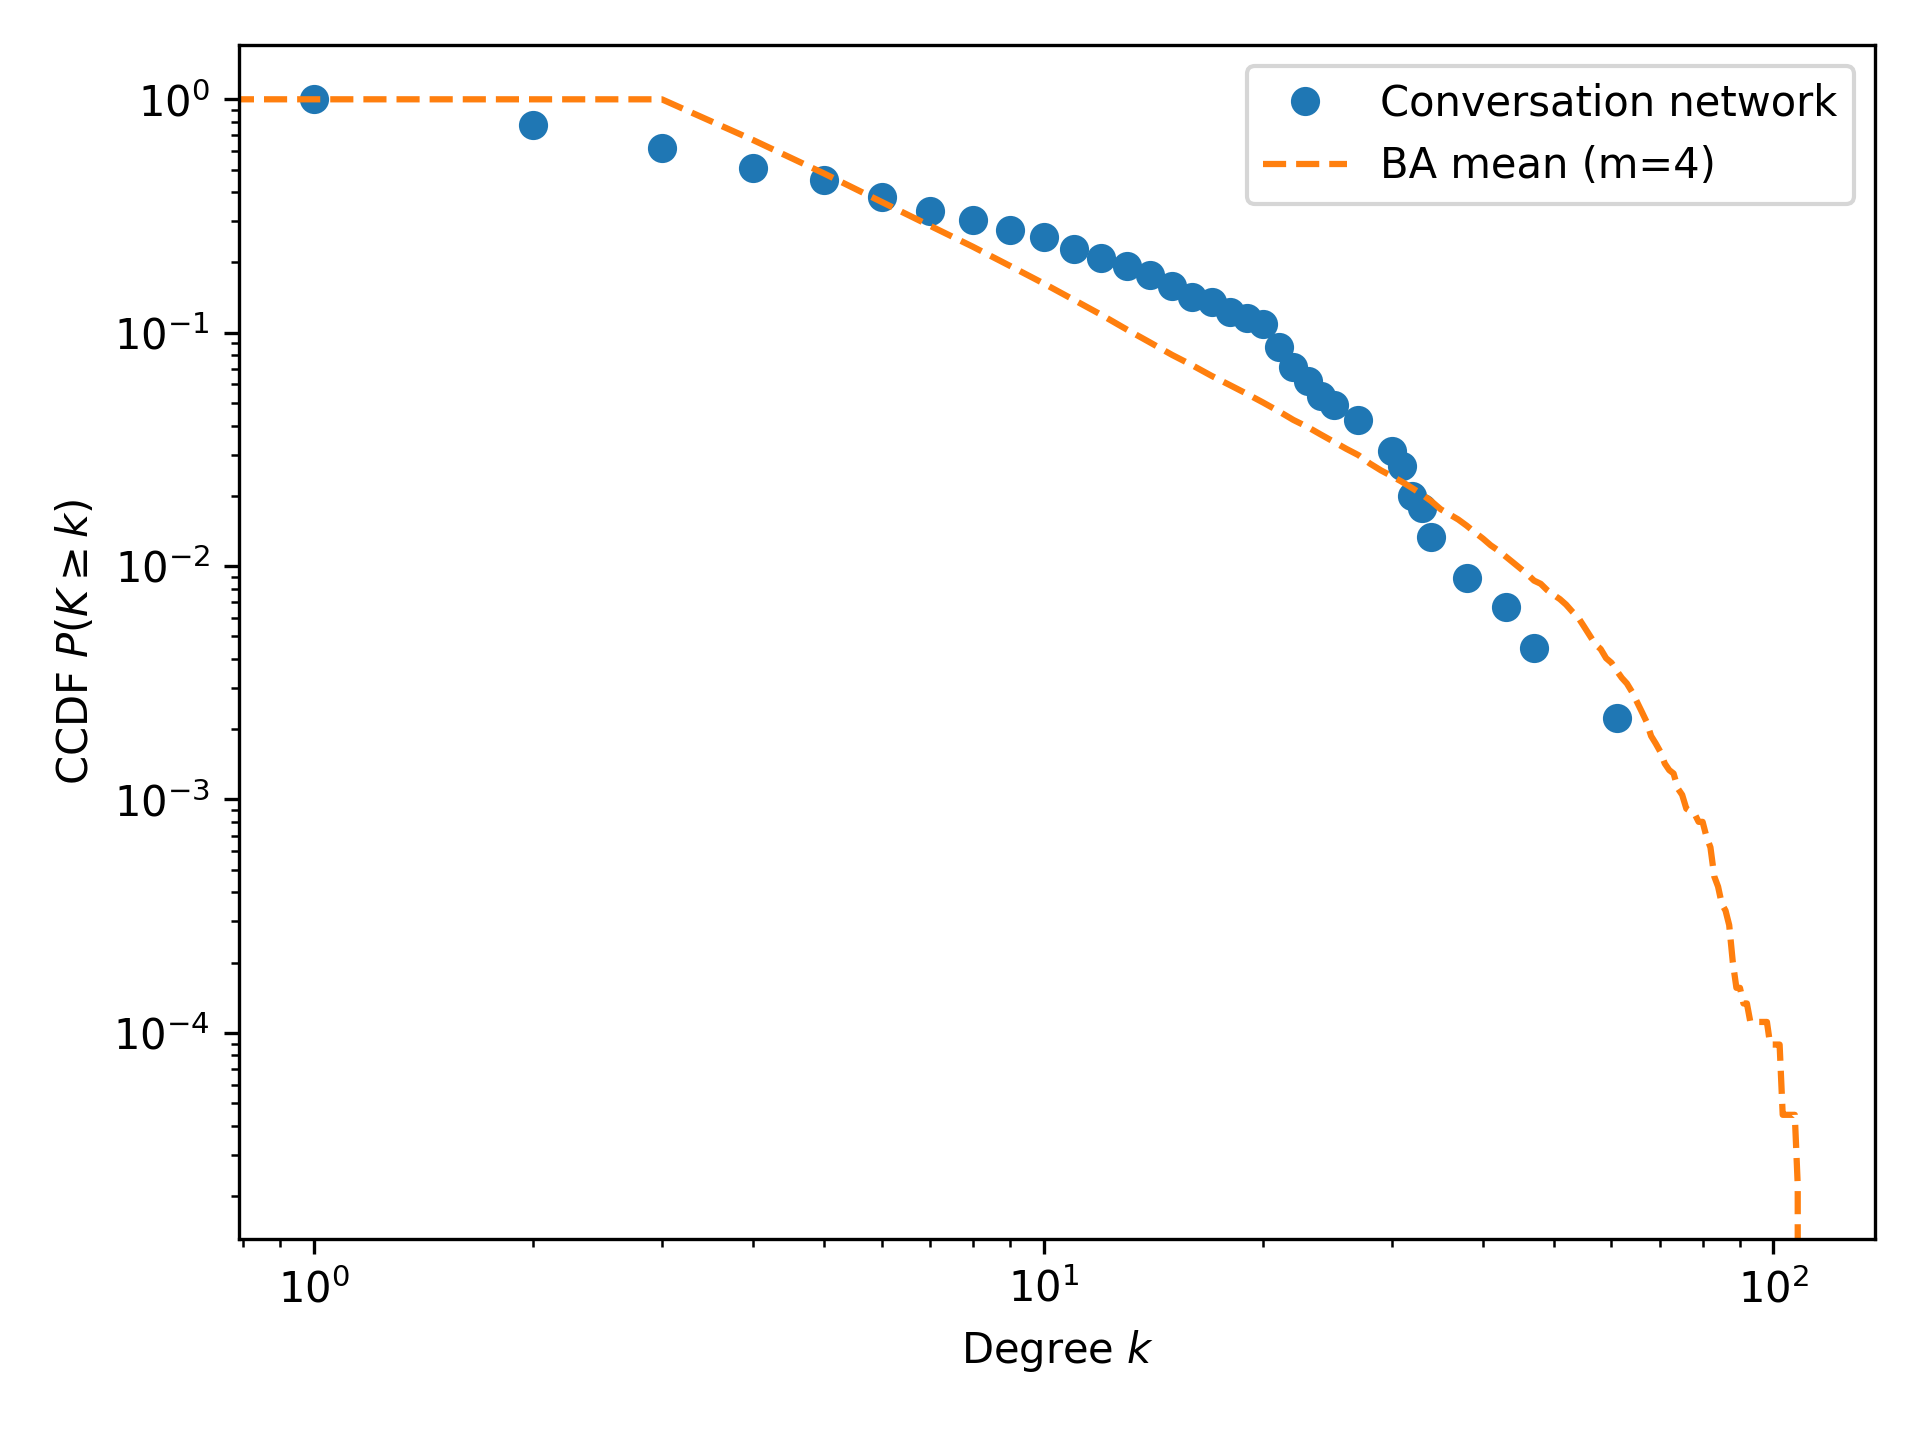
\includegraphics[width=0.82\linewidth]{images/degree_overlay.png}
  \caption{Log--log complementary cumulative degree distribution (CCDF) comparing the conversation network and the mean of 100 BA realisations ($m=4$). The empirical tail steepens significantly beyond $k\approx20$.}
  \label{fig:deg-ccdf}
\end{figure}

Figure~\ref{fig:box-ba} presents box-and-whisker plots for weighted local clustering and average shortest path length. Empirical values are overlaid in red. Table~\ref{tab:ba-metrics} quantifies the differences. From these metrics, we conclude that our conversation network exhibits significant deviations from the BA model, indicating that simple preferential attachment alone cannot account for the observed structure. The empirical network shows:

\begin{enumerate}[label=(\alph*)]
    \item \textbf{Semantic closure:} Clustering in our network is over 14x higher than in the BA baseline (0.593 vs. 0.040), indicating tight topical communities rather than random connections.
    \item \textbf{Longer semantic chains:} The average path length (5.81 vs. 2.93) is nearly double the BA expectation, suggesting meaningful cognitive distance between knowledge domains.
    \item \textbf{Suppressed hub growth:} The degree distribution tail is steeper ($\gamma = 4.7$ vs. $\gamma \approx 3.0$), indicating semantic constraints on unlimited hub formation.
  \end{enumerate}
  
\begin{table}
\centering
\begin{tabular}{lcc}
\toprule
Metric & Conversation & BA mean $\pm$ 95\% CI \\
\midrule
Weighted local clustering $C$ & \textbf{0.593} & $0.040 \pm 0.006$ \\
Average path length $\langle \ell \rangle$ & \textbf{5.81} & $2.93 \pm 0.08$ \\
Diameter & \textbf{18} & 7--9 \\
\bottomrule
\end{tabular}
\caption{Comparison of empirical metrics vs. BA ensemble. Weighted local clustering uses the Onnela definition.}
\label{tab:ba-metrics}
\end{table}

\begin{figure}
    \centering
    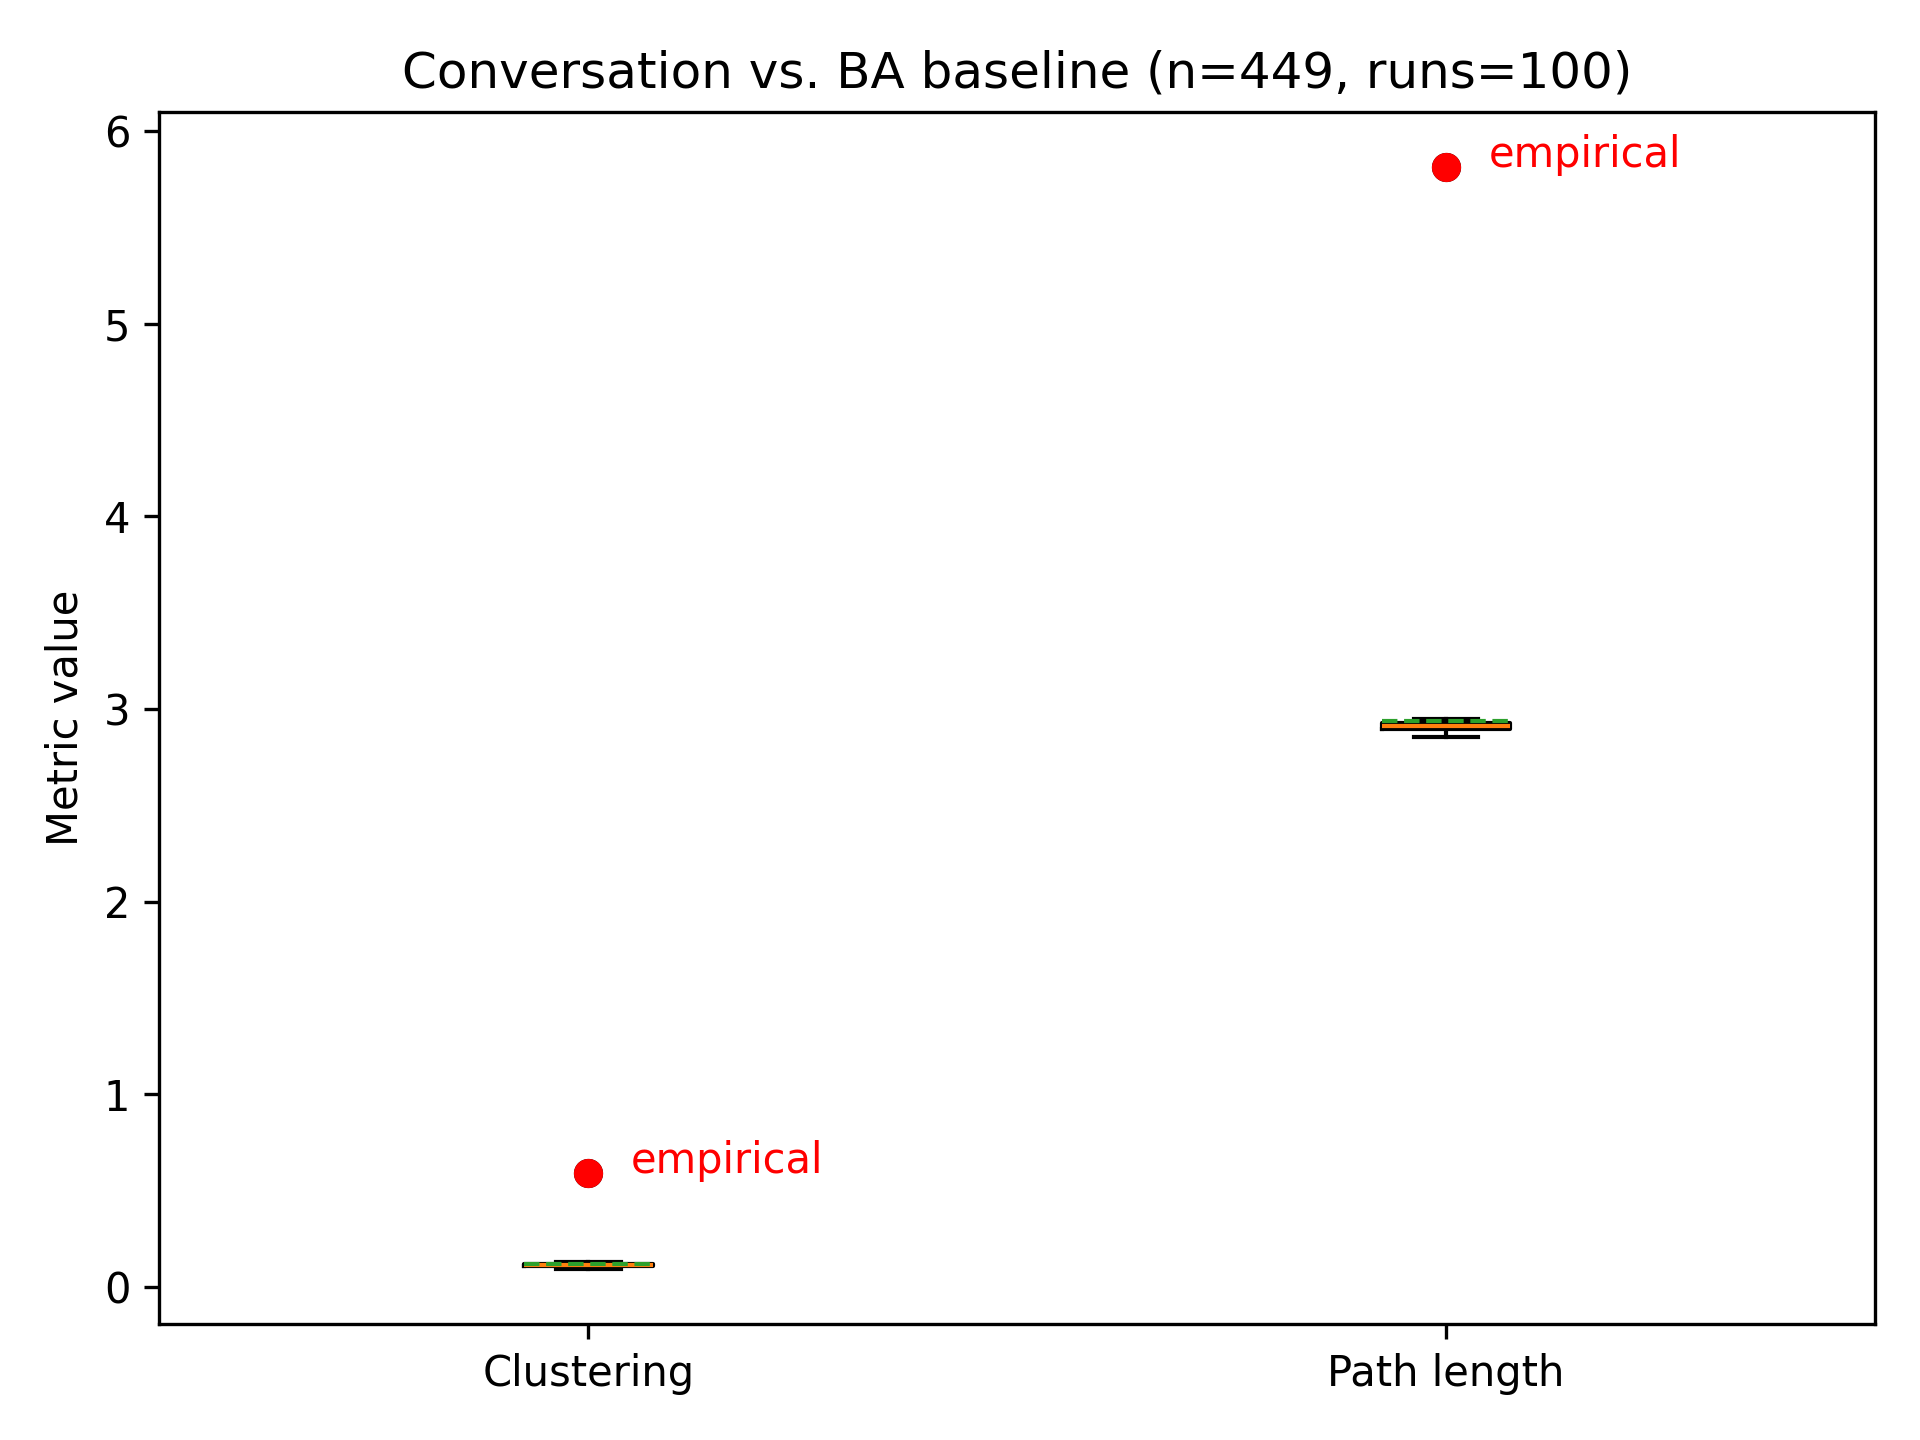
\includegraphics[width=0.75\linewidth]{images/metrics_boxplot.png}
    \caption{Boxplot of clustering coefficient and average path length for 100 Barabási–Albert random graphs compared to our conversation network (red points). The conversation network shows significantly higher clustering and longer path lengths than would be expected from preferential attachment alone, indicating semantic constraints shape network evolution beyond simple preferential attachment mechanisms.}
    \label{fig:box-ba}
\end{figure}


\section{Application: Network-Aware Conversation Recommendation}

Our network analysis reveals structural properties that can be leveraged to enhance conversation recommendation beyond simple semantic similarity. Traditional recommendation systems typically rely solely on content similarity, which can lead to topic siloing and missed opportunities for cross-domain insights. Here, we implement a hybrid recommendation approach that incorporates both semantic similarity and network position.

\subsection{Approach}

We developed a recommendation algorithm as part of our \emph{ChatGPT Complex Net} project \cite{chatgpt-complex-net} that ranks past conversations \(c_i\) for relevance to a new conversation \(c_{\text{cur}}\) using:

\[
  \mathit{score}(c_i)
    = \alpha\,\cos(e_{\text{cur}},e_i)\;
      +\;\beta\,\mathrm{BC}_{\text{norm}}(c_i)
\]

Where:
\begin{itemize}
    \item \(\cos(e_{\text{cur}},e_i)\) is the cosine similarity between the embeddings of the current and candidate conversations
    \item \(\mathrm{BC}_{\text{norm}}(c_i)\) is the normalized betweenness centrality of the candidate conversation
    \item \(\alpha\) and \(\beta\) are tunable parameters that control the balance between similarity and bridging potential
\end{itemize}

This formulation allows users to tune between pure similarity (\(\alpha \gg \beta\)), which returns the most topically relevant conversations, and bridge-awareness (\(\beta\) comparable to \(\alpha\)), which surfaces conversations that connect different knowledge domains and may offer unexpected insights.

\subsection{Example and Results}

To demonstrate this approach, we applied our algorithm to recommend relevant past conversations for a new query about Bayesian statistics:

\begin{tcolorbox}[title=User Prompt]
I want to use a Bayesian approach, where I start with \( X \sim \text{Bernoulli}(p) \), with a prior \( p \sim \text{Beta}(1,1) \), but as more data comes in I expect \( p \to 1 \) in probability. I think I want to create a prior over the convergence of the distribution?
\end{tcolorbox}

\begin{tcolorbox}[title=ChatGPT Response (Excerpt)]
The Bayesian approach updates beliefs via the posterior. With \( p \sim \text{Beta}(1,1) \), you're starting uniform. As data accumulates, posterior becomes more concentrated.

But if you expect \( p \to 1 \), you're implying either a dynamic model or a time-dependent prior. One approach: a sequence of Beta priors with growing skew toward 1. More formally, you could use a \textbf{Bayesian time series} model with \textbf{discounting}...
\end{tcolorbox}

Running our recommendation algorithm with \(\alpha=2, \beta=1\) yielded the results in Table~\ref{tab:recommendations}.

\begin{table}
\centering
\caption{Network-Aware Recommendation Results}
\label{tab:recommendations}
\begin{tabular}{rllrr}
\toprule
Rank & Conversation & Sim & BC$_\text{norm}$ & Score \\
\midrule
1 & r-code-for-ad & 1.000 & 0.000 & 1.9998 \\
2 & training-llms-in-external-tools & 1.000 & 0.000 & 1.9997 \\
3 & latent-code-and-output-for-enriched-context & 0.998 & 0.000 & 1.9959 \\
4 & bias-analysis-in-simulation & 0.989 & 0.0055 & 1.9834 \\
5 & ad-for-mle-with-femtograd & 0.985 & 0.000 & 1.9691 \\
6 & compute-coverage-by-quantile & 0.978 & 0.0001 & 1.9565 \\
7 & hmm-for-data-generation & 0.969 & 0.0017 & 1.9387 \\
8 & variable-t-pdf-calculation & 0.952 & 0.000 & 1.9043 \\
9 & geometric-mean-calculation & 0.442 & 1.000 & 1.8847 \\
\bottomrule
\end{tabular}
\end{table}

\subsection{Discussion of Results}

The results demonstrate several important aspects of our network-aware recommendation approach:

\begin{itemize}
    \item The top recommendations (ranks 1-8) show high semantic similarity to the query, addressing the immediate informational need with closely related conversations.
    
    \item Despite having much lower semantic similarity (0.442), the \textit{geometric-mean-calculation} conversation appears at rank 9 due to its exceptionally high betweenness centrality (1.000). As previously identified in our network analysis, this conversation connects multiple knowledge domains including statistics, probability theory, and machine learning concepts.
    
    \item By incorporating betweenness centrality, the system surfaces this critical bridge conversation that might otherwise be excluded from a purely similarity-based recommendation (which would typically use a minimum similarity threshold well above 0.442).
\end{itemize}

The parameters \(\alpha\) and \(\beta\) provide a simple control mechanism for users to dial between \emph{familiarity} (\(\alpha\gg\beta\)), which prioritizes closely related content, and \emph{bridging} (\(\beta\) comparable to \(\alpha\)), which introduces potential for creative connections across knowledge domains. This approach demonstrates how network structural properties can enhance traditional content-based recommendation systems to support both focused learning and cross-domain knowledge discovery.

In practice, this network-aware recommendation system could be integrated into conversational AI interfaces to help users leverage their conversation history more effectively, supporting both depth-first knowledge exploration within domains and breadth-first discovery across domains.

While this approach shows promise, we acknowledge certain limitations. The effectiveness depends on having sufficiently rich conversation history to form a meaningful network, making it less effective for new users. Additionally, the optimal balance between similarity and betweenness ($\alpha$ and $\beta$ parameters) may vary by domain and user preference, suggesting the need for adaptive tuning mechanisms in practical implementations.

\section{Discussion}

\subsection{Cognitive Interpretation}

The heavy clustering plus truncated-hub behaviour mirrors how humans
explore ideas: intense local rumination punctuated by occasional
cross-topic jumps. In aggregate, the graph becomes a
\emph{structural trace of thinking}---a cognitive MRI---rather than a
social or citation network.  This distinction matters for AI design:
surfacing low-degree, high-betweenness ``pure bridges'' could nurture
creative leaps in real-time dialogue systems.

The deviation from a standard scale-free model suggests multiple mechanisms at work in the growth of conversation networks:

\begin{itemize}
    \item \textbf{Interest-driven attachment}: Users revisit topics of interest, creating hubs
    \item \textbf{Exploration tendency}: Regular venturing into new, unrelated topics
    \item \textbf{Cognitive associations}: Connections based on the user's mental models
\end{itemize}

Unlike citation or social networks, conversation networks appear to more closely reflect cognitive processes of knowledge exploration, with both focused deepening within domains and occasional cross-domain leaps.

\subsection{Community Structure as Knowledge Organization}

The emergence of distinct communities with different internal structures suggests natural knowledge categorization. Particularly interesting is the co-existence of:

\begin{itemize}
    \item Densely connected, high-clustering communities (e.g., community \emph{Stats \& Probability})
    \item Broadly connected, lower-clustering communities (e.g., community \emph{ML/AI/LLM Theory})
    \item Sparsely connected, practical communities (e.g., community \emph{Programming Projects})
\end{itemize}

This variety suggests different conversation types: exploratory conversations that establish broad connections across topics, deep-dive conversations that build dense expert knowledge, and practical conversations focused on specific implementation details.

\subsection{Limitations and Future Research Directions}

Our analysis has several limitations that suggest promising directions for future work:

\begin{itemize}
    \item \textbf{Single-user dataset:} Our analysis is based on a single user's conversation history, limiting generalizability. Future work should extend this methodology to analyze conversation networks from diverse users to understand how different cognitive styles, educational backgrounds, or professional orientations influence knowledge exploration patterns. Comparing networks from mathematics majors versus humanities scholars, for instance, might reveal disciplinary differences in exploration strategies and bridge formation.
    
    \item \textbf{Static network representation:} While our dataset contains complete temporal metadata and we've developed tooling to process it, the current analysis focuses on a static representation of the network. Future research should leverage this existing temporal data to analyze how the network grows and evolves over time by constructing time-slice networks. This would reveal how knowledge domains form organically and how users' interests evolve over extended periods.
    
    \item \textbf{Similarity threshold constraints:} The 0.9 similarity threshold may exclude meaningful weaker connections, as shown in our sensitivity analysis. While this threshold provided clearer community visualization, exploring dynamic thresholding approaches could reveal multi-scale network structures. An illustrative example emerged when using the lower 0.875 threshold: a distinct community formed comprising conversations conducted by or with the author's 13-year-old niece. These conversations, characterized by more artistic topics and a distinct writing style, remained isolated at the 0.9 threshold but became evident at 0.875. This finding demonstrates how threshold selection can significantly impact the detection of subtle user differences or specialized content domains, particularly when the embedding process weights user inputs heavily. This suggests that multi-layer network analysis with varying thresholds might reveal hierarchical community structures reflecting not just topic variation but also authorship, style, and cognitive patterns.
    
    \item \textbf{Embedding limitations:} The embedding process necessarily loses some contextual nuance in conversations. Our current approach treats each conversation as a weighted average of user and assistant contributions, potentially obscuring temporal dynamics within conversations, evolving conceptual shifts, and interactive patterns. Advanced embedding techniques that capture sequential information (such as conversation flow) or employ hierarchical representation (preserving both turn-level and conversation-level semantics) could better preserve these nuances. Future work could explore domain-adapted embeddings, multi-modal representations incorporating images or code snippets shared in conversations, or hybrid approaches that combine semantic and structural features to better represent the full richness of conversational content.
    
    \item \textbf{Statistical validation:} While we provide bootstrap confidence intervals for key metrics, future work could incorporate more sophisticated null models including configuration models that preserve degree sequences, or implement percolation analysis to identify critical thresholds for network formation. Such analyses would provide deeper insights into the mechanisms driving network structure.
\end{itemize}

\section{Conclusion}

This paper presents a novel application of complex network analysis to ChatGPT conversations, revealing rich structural patterns in AI-assisted knowledge exploration. By modeling conversations as a semantic similarity network, we identified distinct knowledge communities, important bridge conversations, and a core-periphery structure that shapes information flow.

Contrary to universal scale-free expectations, our conversation network exhibits a complex multi-regime degree distribution that likely reflects the cognitive processes underlying topic exploration. The identified structure enables practical applications such as network-aware conversation recommendations.

This approach offers valuable insights into how humans explore knowledge spaces with AI assistance and provides practical tools for managing the growing corpus of AI-assisted conversations. As these systems become increasingly integrated into knowledge work, understanding their network structure will be essential for effective knowledge management and discovery.

\bibliographystyle{IEEEtran}
\begin{thebibliography}{00}

\bibitem{alstott2014} J. Alstott, E. Bullmore, and D. Plenz, "powerlaw: A Python package for analysis of heavy-tailed distributions," PLoS ONE, vol. 9, no. 1, p. e85777, 2014.

\bibitem{baronchelli2013} A. Baronchelli, R. Ferrer-i-Cancho, R. Pastor-Satorras, N. Chater, and M. H. Christiansen, "Networks in cognitive science," Trends in Cognitive Sciences, vol. 17, no. 7, pp. 348-360, 2013.

\bibitem{barabasi2009} A.-L. Barabási, "Scale-free networks: A decade and beyond," Science, vol. 325, no. 5939, pp. 412-413, 2009.

\bibitem{borner2003} K. Börner, C. Chen, and K. W. Boyack, "Visualizing knowledge domains," Annual Review of Information Science and Technology, vol. 37, no. 1, pp. 179-255, 2003.

\bibitem{broido2019} A. D. Broido and A. Clauset, "Scale-free networks are rare," Nature Communications, vol. 10, no. 1, p. 1017, 2019.

\bibitem{callon1983} M. Callon, J.-P. Courtial, W. A. Turner, and S. Bauin, "From translations to problematic networks: An introduction to co-word analysis," Social Science Information, vol. 22, no. 2, pp. 191-235, 1983.

\bibitem{clark1998} A. Clark and D. Chalmers, "The extended mind," Analysis, vol. 58, no. 1, pp. 7-19, 1998.

\bibitem{devlin2019} J. Devlin, M.-W. Chang, K. Lee, and K. Toutanova, "BERT: Pre-training of deep bidirectional transformers for language understanding," in Proc. NAACL-HLT, 2019.

\bibitem{efron1993} B. Efron and R. J. Tibshirani, \emph{An Introduction to the Bootstrap}. New York: Chapman \& Hall, 1993.

\bibitem{hutchins1995} E. Hutchins, \emph{Cognition in the Wild}. Cambridge, MA: MIT Press, 1995.

\bibitem{levy2014} O. Levy and Y. Goldberg, "Neural word embedding as implicit matrix factorization," in Advances in Neural Information Processing Systems, 2014.

\bibitem{mikolov2013} T. Mikolov, I. Sutskever, K. Chen, G. S. Corrado, and J. Dean, "Distributed representations of words and phrases and their compositionality," in Advances in Neural Information Processing Systems, 2013.

\bibitem{motter2002} A. E. Motter, A. P. de Moura, Y.-C. Lai, and P. Dasgupta, "Topology of the conceptual network of language," Physical Review E, vol. 65, no. 6, p. 065102, 2002.

\bibitem{pennington2014} J. Pennington, R. Socher, and C. D. Manning, "GloVe: Global vectors for word representation," in Proc. EMNLP, 2014.

\bibitem{price1965} D. J. de S. Price, "Networks of scientific papers," Science, vol. 149, no. 3683, pp. 510-515, 1965.

\bibitem{serban2016} I. V. Serban, R. Lowe, P. Henderson, L. Charlin, and J. Pineau, "A survey of available corpora for building data-driven dialogue systems," arXiv preprint arXiv:1512.05742, 2016.

\bibitem{stella2018} M. Stella, N. M. Beckage, and M. Brede, "Multiplex lexical networks reveal patterns in early word acquisition in children," Scientific Reports, vol. 7, no. 1, pp. 1-10, 2018.

\bibitem{venkatesh2018} A. Venkatesh et al., "On evaluating and comparing conversational agents," arXiv preprint arXiv:1801.03625, 2018.

\bibitem{wegner1987} D. M. Wegner, "Transactive memory: A contemporary analysis of the group mind," in \emph{Theories of Group Behavior}, pp. 185-208, Springer, 1987.

\bibitem{zeng2019} Z. Zeng, H. Deng, X. Guo, and H. Wang, "Topic modeling for short texts with insider and outsider word separation," in Proc. IEEE Int. Conf. on Big Data, 2019.

\bibitem{ctk2024} A. Towell, "conversation-tk: A tool for conversation data extraction and processing," 2024. [Online]. Available: \url{https://github.com/queelius/ctk}. DOI: \url{https://doi.org/10.5281/zenodo.15314402}. PyPi: \url{https://pypi.org/project/conversation-tk/}

\bibitem{chatgpt-complex-net} A. Towell, "chatgpt-complex-net: Complex network analysis of ChatGPT conversations," 2025. [Online]. Available: \url{https://github.com/queelius/chatgpt-complex-net}. DOI: \url{https://doi.org/10.5281/zenodo.15314235}

\end{thebibliography}

\end{document}



